%-----------------------------------------------------------------------------%
\chapter{\babDua}
\label{bab:2}
%-----------------------------------------------------------------------------%
Bab kedua ini menjelaskan mengenai studi literatur yang telah penulis telusuri dan kaji untuk penelitian ini. Sub-bab 2.1 menjelaskan mengenai \emph{natural language processing}, bidang luas yang menjadi domain penelitian ini. Sub-bab 2.2 menjelaskan tentang sistem tanya jawab, \emph{question answering task}, bidang khusus yang menjadi domain penelitian ini. Sub-bab 2.3 menjelaskan tentang \emph{dataset} sistem tanya jawab, \emph{dataset} tersebut ada yang berbahasa Indonesia maupun berbahasa Inggris. Sub-bab 2.4 menjelaskan tentang \emph{natural language inference}, salah satu alat (\emph{tools}) eksperimen untuk meningkatkan performa dari sistem tanya jawab. Sub-bab 2.5 menjelaskan tentang IndoNLI, \emph{dataset natural language inference} berbahasa Indonesia. Sub-bab 2.6 menjelaskan tentang \emph{transformer}, salah satu arsitektur model kecerdasan buatan terbaru untuk dapat memprediksi suatu jawaban. Sub-bab 2.7 menjelaskan tentang arsitektur model yang digunakan pada penelitian ini. Sub-bab 2.8 menjelaskan tentang eksplorasi \emph{dataset} yang akan digunakan. Sub-bab 2.9 dan sub-bab 2.10 menjelaskan tentang \emph{intermediate-task transfer learning} dan \emph{task recasting}, yaitu metode-metode eksperimen yang akan dilakukan pada penelitian ini. Terakhir, sub-bab 2.11 menjelaskan tentang metrik evaluasi yang digunakan pada penelitian ini.

%-----------------------------------------------------------------------------%
\section{Sistem Tanya Jawab (\emph{Question Answering System})}
%-----------------------------------------------------------------------------%

\begin{figure}[h]
\vspace{3pt}
\hrule
\vspace{3pt}

\textbf{\emph{Context}}: Otranto adalah kota dan komune yang terletak di  \colorbox{BurntOrange}{provinsi Lecce} (\colorbox{ForestGreen}{Apulia, Italia}). Otranto berada di pantai timur semenanjung Salento. Selat Otranto menghubungkan Laut Adriatik dengan Laut Ionia. Pelabuhan kota ini kecil dan terdapat sedikit perdagangan.\\

\textbf{\emph{Question}}: \colorbox{BurntOrange}{Dimanakah letak Lecce ?}\\

\textbf{\emph{Answer}}:  \colorbox{ForestGreen}{Apulia, Italia}

\vspace{3pt}
\hrule
\vspace{3pt}
\centering
\caption{Contoh dari \emph{question answering task} dari data \citep{putri-oh-2022-idk}.}
\end{figure}

Sistem tanya jawab merupakan salah satu tugas (\emph{task}) dari domain \emph{Natural Language Processing} (NLP). Sistem tanya jawab adalah sistem yang dirancang untuk memenuhi kebutuhan informasi manusia yang mungkin muncul dalam situasi seperti berbicara dengan asisten virtual, berinteraksi dengan pencarian mesin (\emph{search engine}), atau sekedar menanyakan data di basis data (\emph{database}) saja \citep{daniel2007speech}. Salah satu paradigma pencarian jawaban dari suatu sistem tanya jawab ini adalah dengan berbasis pencarian informasi (\emph{information-retrieval-based}). Arti dari berbasis pencarian informasi di atas adalah: mesin diberikan suatu informasi (nanti disebut sebagai konteks) dan suatu pertanyaan, dan mesin sistem tanya jawab menggunakan metode pencarian informasi untuk menentukan bagian teks yang relevan dengan pertanyaan yang diberikan, dengan menggunakan algoritma dari \emph{machine reading comprehension} (MRC) mesin sistem tanya jawab dapat menemukan jawaban dari bagian teks tersebut dengan mengambil kalimat (\emph{span of text}) yang kemungkinan besar menjadi jawabannya; mesin sistem tanya jawab dengan berbasis pencarian informasi ini bergantung pada kumpulan teks yang besar agar mesin menjadi lebih akurat. 

Jenis-jenis tugas (\emph{task}) yang dapat diselesaikan oleh suatu sistem tanya jawab, antara lain: \emph{factoid question answering} dimana pertanyaan dapat dijawab dengan fakta sederhana yang dapat dituliskan dalam teks pendek, lalu \emph{long-form question answering} dimana pertanyaan dapat dijawab dengan kalimat yang panjang, biasanya pertanyaan “mengapa”; kemudian \emph{community question answering} dimana pasangan tanya jawab didapatkan dari suatu komunitas seperti Quora, dan lain sebagainya. Tugas-tugas yang dapat diselesaikan oleh sistem tanya jawab bisa bertambah varian dan ragamnya seiring dengan pesatnya riset dan pengembangan di bidang NLP.

%-----------------------------------------------------------------------------%
\section{\emph{Dataset} Umum Pada Sistem Tanya Jawab}
%-----------------------------------------------------------------------------%
Pada bagian ini, akan dipaparkan berbagai macam \emph{dataset} yang biasa dan umum digunakan pada pengembangan suatu sistem tanya jawab.

%-----------------------------------------------------------------------------%
\subsection{SQuAD}
%-----------------------------------------------------------------------------%
\emph{Stanford Question Answering Dataset} atau disingkat dengan SQuAD (versi 1.1) merupakan suatu kumpulan data (\emph{dataset}) yang berisi pasangan dari 100.000 lebih pertanyaan dan jawaban \citep{rajpurkar-etal-2016-squad}. Pertanyaan diajukan kepada anotator dari sebuah konteks dari halaman Wikipedia, yang dimana jawabannya harus dapat diekstrak dari konteks halaman Wikipedia tersebut. Konteks tersebut dipilih dari 536 halaman Wikipedia. Bentuk jawaban beragam dan butuh alasan (\emph{reasoning}) untuk dapat menjawabnya. Alur pengumpulan data dilakukan dalam alur sebagai berikut: pencarian 10.000 halaman teratas pada Wikipedia, lalu dilakukan pengambilan contoh/sampel (\emph{sampling}) sebanyak 536 halaman, lalu dari halaman-halaman tersebut ditanyakan kepada anotator untuk dicari jawabannya, terakhir; untuk evaluasi model yang lebih kokoh (\emph{robust}) maka dicari lagi anotator baru untuk menambahkan jawaban baru pada sebagian pertanyaan.

Saat ini, SQuAD sudah sampai versi 2.0, perbedaan SQuAD versi ini dengan sebelumnya adalah penambahan 50.000 soal yang tidak dapat dijawab (\emph{unanswerable question}) dari konteks halaman Wikipedia yang telah diberikan \citep{rajpurkar-etal-2018-know}. Hal tersebut dilakukan untuk memaksa model pembelajaran mesin (\emph{machine learning}) agar dapat menjawab “tidak ada jawaban” dibanding dengan harus mengarang jawaban yang sebenarnya tidak ada pada konteks yang diberikan. SQuAD sudah menjadi tolak ukur (\emph{benchmark}) dalam penilaian evaluasi dari suatu sistem tanya jawab (\emph{question answering system}).

%-----------------------------------------------------------------------------%
\subsection{TyDi-QA}
%-----------------------------------------------------------------------------%
\emph{Typologically Diverse Languages Question Answer} atau disingkat dengan TyDi-QA merupakan suatu kumpulan data (\emph{dataset}) yang berisi pasangan dari 204.000 lebih pertanyaan dan jawaban dalam 11 bahasa yang beragam secara tipologis \citep{clark-etal-2020-tydi}. Tujuan dari penggunaan bahasa yang beragam ini agar dapat menangkap beragam fenomena bahasa dan fenomena linguistik yang tidak ditemukan pada dokumen yang hanya memiliki bahasa Inggris saja. Kemudian, menurut \citet{clark-etal-2020-tydi} \emph{dataset} TyDi-QA ini lebih berkualitas dan realistis, sebab anotator yang menulis pertanyaan memang benar-benar ingin tahu jawaban dari suatu petunjuk tema (\emph{prompt}) yang diberikan, bukan sekadar menulis pertanyaan sederhana yang jawabannya dengan mudah diekstrak dari petunjuk tema (\emph{prompt}) yang diberikan. Pada \emph{dataset} ini, terdapat \emph{dataset} berbahasa Indonesia, yang terdapat pada \emph{secondary gold passage task dataset} TyDi-QA ini, bagian ini yang \citet{cahyawijaya-etal-2021-indonlg} sebut sebagai TyDi-QA-ID , dengan pembagian 15\% dari data pelatihan (\emph{training}) digunakan sebagai set pengujian (\emph{testing}).

Alur pengumpulan data dilakukan dalam alur sebagai berikut: anotator diberikan sebuah petunjuk tema (\emph{prompt}) dari halaman Wikipedia yang berisi 100 karakter pertama dari halaman tersebut, lalu anotator diminta untuk menulis pertanyaan (yang benar-benar ingin diketahui atau yang tidak dapat terjawab) dari petunjuk tersebut, kemudian dicarikan artikel Wikipedia lainnya untuk dapat menjawab pertanyaan tersebut, jika ditemukan jawaban di artikel tersebut, maka akan dilakukan pelabelan jawaban (\emph{answer labelling}) oleh anotator \citep{clark-etal-2020-tydi}. Sebelas bahasa yang dikumpulkan itu memang benar-benar dikumpulkan dalam bahasa aslinya, bukan penerjemahan dari bahasa yang satu ke bahasa yang lainnya, agar dapat menjaga urutan bahasa asli tersebut yang akhirnya akan bisa menangkap fenomena bahasa dan fenomena linguistik yang lebih beragam dan realistis. Harapan \citet{clark-etal-2020-tydi} adalah \emph{dataset} TyDi-QA ini menjadi tolak ukur (\emph{benchmark}) untuk sistem tanya jawab yang setidaknya dapat digunakan oleh 100 bahasa dengan penutur terbanyak.

%-----------------------------------------------------------------------------%
\subsection{IDK-MRC}
%-----------------------------------------------------------------------------%
\emph{I Don’t Know Machine Reading Comprehension} atau yang disingkat dengan IDK-MRC merupakan suatu kumpulan data (\emph{dataset}) yang berisi dengan 5.000 lebih pertanyaan dan jawaban berbahasa Indonesia yang mayoritas pertanyaannya sengaja agar tidak bisa dijawab (\emph{unanswerable}) dari konteks yang diberikan \citep{putri-oh-2022-idk}. Sebenarnya ide pembuatan \emph{dataset} ini mirip dengan ide \emph{dataset} SQuAD versi 2.0, yang bertujuan untuk memaksa model pembelajaran mesin (\emph{machine learning}) agar dapat menjawab “tidak ada jawaban” dibandingkan harus mengarang jawaban. Namun karena SQuAD tidak memfasilitasi bahasa Indonesia, maka IDK-MRC dapat menjadi solusinya. \emph{Dataset} IDK-MRC ini dibangun di atas hasil penerjemahan dari SQuAD versi 2.0.

Alur pengumpulan data dilakukan dalam alur sebagai berikut: awalnya akan dihasilkan pertanyaan yang tidak terjawab (\emph{unanswerable question}) dari mesin \emph{question generation} (QG) yang dipicu dari sebuah sampel konteks, pertanyaan, dan jawaban yang diberikan, lalu dilakukan penyaringan agar pertanyaan tersebut dapat lebih masuk akal untuk ditanyakan walaupun juga tidak terdapat jawabannya, lalu dilakukan pengecekan kemiripan dengan pertanyaan yang dapat dijawab agar pertanyaan yang tidak dapat dijawab dapat lebih relevan untuk ditanyakan, lalu akan dicek secara manual oleh anotator nilai relevansi pertanyaan tersebut dan akan dihasilkan (\emph{generate}) lagi pertanyaan yang tidak dapat terjawab secara manual agar dapat mengatasi permasalahan sulitnya mesin \emph{question generation} (QG) untuk dapat menghasilkan pertanyaan yang tak dapat terjawab dari sebagian tipe-tipe pertanyaan yang ada \citep{putri-oh-2022-idk}.

%-----------------------------------------------------------------------------%
\subsection{SQuAD-ID}
%-----------------------------------------------------------------------------%
\emph{Stanford Question Answering Dataset Indonesia} atau yang disingkat dengan SQuAD-ID merupakan kumpulan data (\emph{dataset}) yang berisi pasangan dari 100.000 lebih pertanyaan dan jawaban dalam bahasa Indonesia yang terdapat juga pertanyaan yang tidak terjawab di dalamnya \citep{muis2020sequencetosequence}. Mirip dengan \emph{dataset} IDK-MRC, \emph{dataset} SQuAD-ID juga merupakan hasil penerjemahan dari \emph{dataset} SQuAD versi 2.0, namun pada \emph{dataset} SQuAD-ID penerjemahan dilakukan secara otomatis, tidak menggunakan penerjemahan manual oleh anotator yang dimana \emph{dataset} IDK-MRC melakukannya. Otomasi penerjemahan \emph{dataset} SQuAD yang berbahasa Inggris menjadi SQuAD yang berbahasa Indonesia dilakukan dengan metode: \emph{Sequence-to-Sequence Learning}. Pemilihan metode tersebut dikarenakan metode tersebut adalah \emph{state-of-the-art} dari pembuatan model \emph{Automatic Question Generator} (AQG). 

Alur pengumpulan data dilakukan dalam alur sebagai berikut: penerjemahan \emph{dataset} SQuAD secara kasar terlebih dahulu, lalu terjemahan tersebut dilakukan pra proses (\emph{preprocessing}), lalu terjemahan tersebut digunakan untuk suplai model \emph{sequence-to-sequence learning} yang sudah dibangun, lalu hasil prediksi dari model \emph{sequence-to-sequence learning} tersebut akan dievaluasi sebagai bagian dari evaluasi model (\emph{model evaluation}), agar model \emph{sequence-to-sequence learning} tersebut dapat lebih akurat menerjemahkan \emph{dataset} SQuAD-nya.

%-----------------------------------------------------------------------------%
\section{\emph{Natural Language Inference}}
%-----------------------------------------------------------------------------%

\begin{figure}[h]
\vspace{3pt}
\hrule
\vspace{3pt}

\textbf{\emph{Premise}}: Selanjutnya, dua pemain Arsenal yang dirasa Ian Wright kurang sip adalah di sektor serang. Mereka adalah Willian dan Alexandre Lacazette, yang disebutnya buntu.\\

\textbf{\emph{Hypothesis}}: Alexandre Lacazette tidak memiliki performa yang baik sebagai penyerang.\\

\textbf{\emph{Label}}:  \emph{Entailment}

\vspace{3pt}
\hrule
\vspace{3pt}

\textbf{\emph{Premise}}: Seakan tak bisa dipisahkan, dua sahabat itu sama-sama sedang menggarap proyek musik.\\

\textbf{\emph{Hypothesis}}: Dua sahabat itu selalu bersama-sama.\\

\textbf{\emph{Label}}:  \emph{Neutral}

\vspace{3pt}
\hrule
\vspace{3pt}

\textbf{\emph{Premise}}: Meskipun trikomoniasis adalah penyakit yang sangat umum, penyakit ini seringkali sulit diketahui.\\

\textbf{\emph{Hypothesis}}: Trikomoniasis bukanlah penyakit yang umum.\\

\textbf{\emph{Label}}:  \emph{Contradiction}

\vspace{5pt}
\hrule
\vspace{5pt}

\centering
\caption{Contoh dari \emph{natural language inference} dari data IndoNLI \citep{mahendra-etal-2021-indonli}.}
\end{figure}

\emph{Natural Language Inference} atau disingkat dengan NLI merupakan suatu tugas semantik (\emph{semantic task}) pada domain NLP yang bertujuan untuk mengkarakterisasi dan memanfaatkan relasi antar dua kalimat, untuk menyelesaikan hal tersebut, model membutuhkan kemampuan untuk mengurai semantik kalimat dan penalaran logis (\emph{commonsense}) yang baik \citep{bowman-etal-2015-large}. Permasalahan NLI ini dapat diselesaikan dengan berbagai teknik, seperti: menggunakan logika simbolis (\emph{symbolic logic}), menggunakan logika pengetahuan umum (\emph{knowledge-based}), dan yang paling baru adalah dengan menggunakan \emph{neural networks}. 

Sekarang, NLI sudah dijadikan menjadi tolak ukur (\emph{benchmark}) dalam bidang representasi semantik dari suatu kalimat. Sudah banyak \emph{dataset} pengujian NLI ini, antara lain seperti: \emph{Stanford Natural Language} Inference (SNLI), \emph{Multi-Genre Natural Language Inference} (MultiNLI) yang dapat digunakan sebagai bahan pengujian dari suatu sistem NLI. MultiNLI merupakan \emph{dataset} yang lebih baru dibandingkan dengan SNLI dengan penambahan ragam genre tema kalimat \citep{williams-etal-2018-broad}. Pengaplikasian NLI ini masih relevan dengan permasalahan sistem tanya jawab, NLI dapat diaplikasikan sebagai \emph{intermediate task transfer learning}, validasi prediksi jawaban, dan bisa juga menghasilkan (\emph{generate}) prediksi jawaban dengan melakukan pra proses (\emph{preprocess}) terlebih dahulu.

Kemudian, salah satu \emph{dataset} NLI berbahasa Indonesia yang dapat digunakan sebagai bahan eksperimen adalah IndoNLI. IndoNLI merupakan \emph{dataset} NLI pertama yang diperoleh dari manusia (bukan dari mesin otomatis) dengan berbahasa Indonesia. Pada \emph{dataset} ini terdapat sekitar 18 ribu lebih pasangan kalimat yang dianotasi \citep{mahendra-etal-2021-indonli}; \emph{dataset} ini dianotasi oleh dua kelompok individu, yaitu: individu biasa yang jumlahnya lebih banyak (\emph{lay annotator}), dan para pakar dalam bidang NLP (\emph{expert annotator}). Ada beberapa bagian dari data yang sengaja dijadikan data uji coba (\emph{test bed}) dengan memasukkan beragam fenomena linguistik, seperti: penalaran numerik (\emph{numerical reasoning}), perubahan struktural kalimat (\emph{structural changes}), idiom, atau penalaran temporal dan spasial (\emph{temporal and spatial reasoning}). Kemudian, menurut \citet{mahendra-etal-2021-indonli} \emph{dataset} IndoNLI yang dianotasi oleh pakar lebih banyak keragamannya (\emph{diverse}) dan memiliki artefak anotasi yang lebih sedikit dibandingkan dengan data yang dianotasi orang banyak.

Alur pengumpulan data IndoNLI mengikuti protokol pengumpulan data \emph{Multi-Genre Natural Language Inference} (MultiNLI), yaitu dilakukan dalam alur sebagai berikut: pengumpulan teks premis dari tiga genre, yaitu dari Wikipedia, berita, dan artikel web; lalu premis-premis tersebut diberikan kepada setiap anotator dan anotator diminta untuk menuliskan enam hipotesis, masing-masing dua label \emph{entailment}, \emph{contradiction}, dan \emph{neutral}; di bagian ini anotator pakar menuliskan fenomena linguistik untuk setiap pasangan premis dan hipotesis; terakhir, dilakukan validasi untuk setiap premis, hipotesis, dan labelnya yang dilakukan secara manual oleh anotator independen lainnya. Harapan \citet{mahendra-etal-2021-indonli}, \emph{dataset} IndoNLI ini dapat membantu mengembangkan kemajuan penelitian dan riset pada bidang NLP di Indonesia.

%-----------------------------------------------------------------------------%
\section{\emph{Transformer}}
%-----------------------------------------------------------------------------%

\begin{figure}[h]
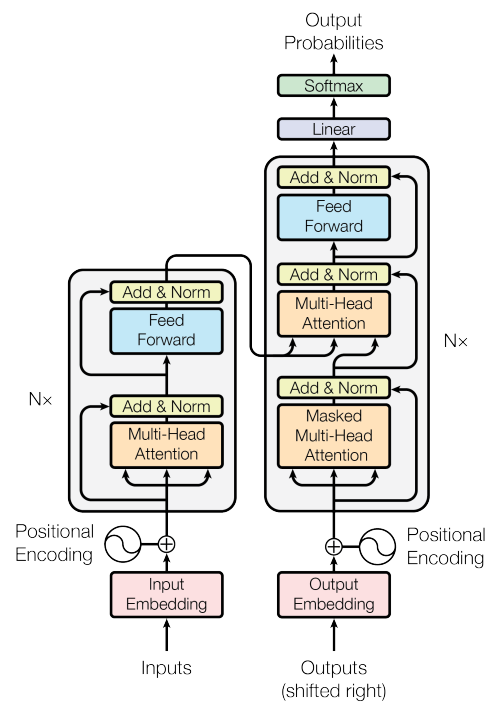
\includegraphics[scale=0.5]{assets/pics/transformer-achitecture.png}
\centering
\caption{Arsitektur model \emph{transformer}.\\\hspace{\textwidth}Referensi gambar: \citep{DBLP:journals/corr/VaswaniSPUJGKP17}}.
\end{figure}

\emph{Transformer} merupakan tipe arsitektur \emph{artificial neural networks} yang digunakan untuk memecahkan masalah transformasi dari urutan masukan (\emph{input}) menjadi urutan keluaran (\emph{output}) dalam suatu aplikasi \emph{deep learning} \citep{transformers-self-attention-to-the-rescue}. Keberadaan Transformer dianggap sebagai solusi dari permasalahan-permasalahan pada \emph{recurrent neural network} (RNN) dan \emph{long short-term memory} (LSTM), yang berkaitan dengan \emph{vanishing \& exploding gradient problem} pada RNN dan keterkaitan antar kata (\emph{relationship between words}) pada LSTM. Cara \emph{transformer} mengatasi masalah-masalah tersebut adalah dengan menggunakan \emph{self-attention}. \emph{Self-attention} merupakan mekanisme perhatian (\emph{attention}) yang menghubungkan posisi yang berbeda dari suatu urutan untuk menghitung representasi urutan tersebut \citep{DBLP:journals/corr/VaswaniSPUJGKP17}; sederhananya \emph{self-attention} merupakan mekanisme yang mempelajari keterkaitan antar kata (\emph{relationship between words}) yang gagal diatasi oleh LSTM. 

Kemudian, alasan mengapa \emph{transformer} dapat mengatasi \emph{vanishing \& exploding gradient problem}, adalah karena \emph{Transformer} tidak bergantung pada perulangan (\emph{recurrent}) seperti yang dilakukan pada RNN, namun \emph{Transformer} bergantung kepada mekanisme perhatian (\emph{attention}) sepenuhnya, sehingga \emph{transformer} dapat terhindar dari perkalian angka-angka gradien kecil maupun besar yang dapat menyebabkan \emph{vanishing \& exploding gradient problem}. Kemudian, \emph{transformer} memungkinkan paralelisasi yang lebih signifikan dari arsitektur-arsitektur lainnya. Hal tersebut yang membuat \emph{Transformer} menjadi \emph{state-of-the-art} model dari perkembangan arsitektur \emph{artificial neural networks} sampai saat ini.

%-----------------------------------------------------------------------------%
\section{\emph{Pre-trained Language Model}}
%-----------------------------------------------------------------------------%
Pada bagian ini, akan dipaparkan berbagai macam \emph{pre-trained language model} yang akan digunakan pada penelitian saat ini. Sederhananya, \emph{pre-trained language model} adalah model bahasa yang telah dilatih terlebih dahulu pada korpus teks yang besar untuk mempelajari pola bahasa dan representasi dari suatu kata. Proses \emph{training} model biasa dilakukan dengan teknik: belajar untuk memprediksi atau menghasilkan kata berikutnya dalam sebuah kalimat berdasarkan konteks kata sebelumnya dan/atau setelahnya (\emph{masked language modelling}) ataupun dengan memprediksi apakah suatu kalimat ada setelah kalimat lainnya (\emph{next sentence prediction}), hal tersebut bertujuan untuk menangkap pola statistik dan hubungan semantik dalam suatu bahasa. Proses ini memungkinkan model untuk mempelajari "\emph{word embeddings}" dan representasi kontekstual yang menyimpan informasi tentang makna kata, struktur sintaksis, dan beragam hal lainnya \citep{radford2018improving}.

%-----------------------------------------------------------------------------%
\subsection{BERT}
%-----------------------------------------------------------------------------%

BERT yang merupakan singkatan dari \emph{Bidirectional Encoder Representations from Transformers} merupakan salah satu \emph{pre-trained language model} yang dikembangkan oleh Google dan secara spesifik bertujuan sebagai representasi suatu bahasa atau dalam kata lain sebagai \emph{language representation models}. BERT sengaja dirancang untuk belajar representasi bahasa secara dua arah, yaitu: kiri ke kanan, dan kanan ke kiri. BERT dapat digunakan sebagai model untuk menjawab pertanyaan (\emph{question answering task}), inferensi bahasa, dan lain-lain \citep{devlin-etal-2019-bert}. Untuk jumlah komponen dalam model BERT itu sendiri, dapat dipaparkan sebagai berikut: untuk jenis BERT-\emph{base}, \emph{layer}-nya sebanyak 12 \emph{layer}, \emph{hidden-size} sebanyak 768, dan banyaknya \emph{self-attention heads} sebanyak 12, dan terakhir, banyaknya parameter sebanyak 110 juta parameter; kemudian untuk jenis BERT-\emph{large}, \emph{layer}-nya sebanyak 24 \emph{layer}, \emph{hidden-size} sebanyak 1024, dan banyaknya \emph{self-attention heads} sebanyak 16, dan terakhir, banyaknya parameter sebanyak 340 juta parameter. BERT sendiri secara orisinil dilatih dengan bahasa Inggris saja, namun, untuk kepentingan penelitian ini, kita menggunakan IndoBERT, yaitu BERT yang dilatih dengan bahasa Indonesia \citep{koto2020indolem}.

Arsitektur dari model BERT itu sendiri mengusung arsitektur \emph{multi-layer bidirectional Transformer encoder}, yaitu: model yang memiliki beberapa \emph{layer} dan bersifat dua arah (\emph{bidirectional}), hal tersebut berbeda dengan kebanyakan arsitektur model yang biasanya bersifat satu arah (\emph{directional}). Menurut 
\citet{devlin-etal-2019-bert} penggunaan sifat \emph{bidirectional} ini ditekankan untuk memahami pentingnya kontribusi sifat \emph{bidirectional} pada keberhasilan performa \emph{training} BERT itu sendiri, karena kelebihan yang dimiliki sifat \emph{bidirectional} dibandingkan dengan sifat \emph{directional} biasa. Karena, menurut \citet{devlin-etal-2019-bert} dengan sifat \emph{bidirectional} akan memungkinkan setiap kata untuk secara langsung untuk dapat melatih kata masing-masing secara independen, dan model dapat dengan mudah memprediksi kata target dalam suatu konteks.

%-----------------------------------------------------------------------------%
\subsection{RoBERTa}
%-----------------------------------------------------------------------------%
RoBERTa yang merupakan singkatan dari \emph{A Robustly Optimized BERT Pretraining Approach} adalah salah satu model yang merupakan suatu \emph{pre-trained language model} pengembangan dari \emph{pre-trained language model} BERT. Modifikasi yang dilakukan oleh \citet{liu2019roberta} pada model BERT antara lain: memperbanyak waktu \emph{training} dengan jumlah \emph{batch} yang lebih besar, menghapus objektif \emph{next-sentence-prediction}, melatih model untuk \emph{sequence} yang lebih panjang, mengubah secara dinamis \emph{masking pattern} pada data latih, dan dilatih dengan \emph{dataset} baru yang lebih besar. 

Alasan mengapa dilakukan modifikasi tersebut adalah karena menurut \citet{liu2019roberta} setelah dilakukan evaluasi terhadap model BERT termasuk \emph{hyperparameters tuning} dan \emph{training set size}, model BERT dianggap \emph{ significantly undertrained} yang menyebabkan hasil performa dari BERT masih dirasa kurang baik oleh \citeauthor{liu2019roberta}. Oleh karena itu \citet{liu2019roberta} mengusulkan resep yang terbukti lebih baik untuk melatih model BERT, yaitu: RoBERTa; yang performanya dianggap setara atau melebihi kinerja semua metode pasca kemunculan model BERT.

%-----------------------------------------------------------------------------%
\subsection{XLM-RoBERTa}
%-----------------------------------------------------------------------------%
XLM-RoBERTa yang merupakan singkatan dari \emph{Cross-lingual Language Model For Robustly Optimized BERT Pretraining Approach} adalah salah satu \emph{pre-trained language model} yang merupakan suatu model pengembangan dari \emph{pre-trained language model} RoBERTa. Modifikasi yang dilakukan oleh \citet{conneau2020unsupervised} pada model RoBERTa adalah penggunaan banyak bahasa pada data latih model XLM-RoBERTa, yang mencakup sekitar 100 bahasa yang disadur dari halaman Wikipedia dengan beragam bahasa yang tersedia. Penggunaan banyak bahasa ini dipengaruhi oleh adanya model mBERT yang menggunakan data latih dari 104 bahasa.

Alasan mengapa dilakukan modifikasi tersebut adalah untuk menguji \emph{cross-lingual language understanding (XLU) task} untuk  memperoleh performa terbaik dalam \emph{task-task} lintas bahasa, seperti: \emph{cross-lingual classification, cross-lingual sequence labeling} dan \emph{cross-lingual question answering}. Karena kebutuhan model untuk \emph{task} lintas bahasa masih banyak dibutuhkan. Apalagi dengan anggapan bahwa dengan \emph{task} lintas bahasa dapat meningkatkan kinerja pada \emph{task} NLP lainnya dengan memanfaatkan struktur linguistik pada beragam bahasa tersebut.

%-----------------------------------------------------------------------------%
\section{\emph{Intermediate-Task Transfer Learning}}
%-----------------------------------------------------------------------------%

\begin{figure}[h]
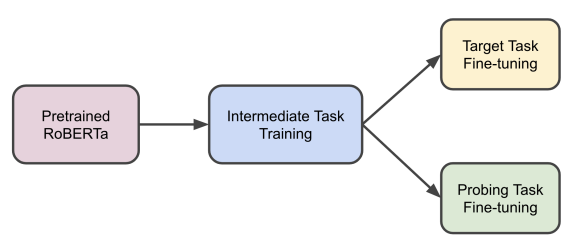
\includegraphics[width=\linewidth]{assets/pics/ittl-pipeline.png}
\centering
\caption{Salah satu contoh alur penggunaan \emph{Intermediate-Task Transfer Learning}.\\\hspace{\textwidth}Referensi gambar: \citep{pruksachatkun-etal-2020-intermediate}.}
\end{figure}

\emph{Intermediate-Task Transfer Learning} merupakan teknik peningkatan performa dengan melakukan \emph{fine-tuning} dengan \emph{dataset} tugas lain (\emph{intermediate task}) pada model \emph{Transformer}, lalu model yang sudah dilakukan \emph{fine-tuning} tersebut akan dilakukan \emph{fine-tuning} kembali untuk tugas tujuannya (\emph{target task}) \citep{pruksachatkun-etal-2020-intermediate}. Harapannya, dengan logis, bila suatu model sudah dilatih pada tugas lain, model tersebut cenderung akan memberikan hasil yang baik bila model yang sudah dilatih tersebut dilatih kembali di tugas yang berbeda, namun masih dalam lingkup domain \emph{task} yang relevan. Teknik \emph{Intermediate-Task Transfer Learning} ini memanfaatkan kelebihan yang terdapat pada arsitektur \emph{Transformer} yang sudah dilatih pada \emph{dataset} yang sangat besar; seharusnya kinerja \emph{Transformer} dapat ditingkatkan dengan melatih model lebih lanjut pada tugas perantara (\emph{intermediate task}) yang memiliki data yang lebih kaya, beragam, dan berkualitas; sebelum melakukan penyempurnaan model pada tugas target (\emph{target task}) via \emph{transfer learning}. 

Namun, menurut \citet{pruksachatkun-etal-2020-intermediate}, masih belum mengetahui kapan dan bagaimana cara tugas perantara (\emph{intermediate task}) mempengaruhi dan bermanfaat bagi tugas target (\emph{target task}). Untuk mengetahui hal tersebut, studi \citet{pruksachatkun-etal-2020-intermediate} menemukan beberapa hal menarik, antara lain: \emph{intermediate task} membutuhkan inferensi tingkat tinggi (\emph{high-level inference}) dan kemampuan penalaran (\emph{reasoning abilities}) yang baik agar dapat bermanfaat bagi tugas targetnya, kemudian kinerja dari tugas target sangat berkorelasi dengan kemampuan inferensi tingkat yang lebih tinggi seperti pengelompokan penyebutan kata dalam teks yang mengacu pada entitas dunia nyata yang sama \citep{coference-resolution}. Contoh dari \emph{intermediate task} yang dapat membantu meningkatkan performa \emph{target task} dari eksperimen \citeauthor{pruksachatkun-etal-2020-intermediate} adalah MNLI dan \emph{commonsense-oriented tasks} seperti CommonsenseQA, HellaSWAG, dan CosmosQA yang terbukti dapat memberikan peningkatan performa yang signifikan kepada sebagian \emph{target task} yang sedang diuji.

%-----------------------------------------------------------------------------%
\section{\emph{Task Recasting}}
%-----------------------------------------------------------------------------%
\emph{Task recasting} merupakan teknik untuk mengubah bentuk \emph{dataset} (atau model), dari satu \emph{task} ke \emph{task} lainnya. \emph{Task recasting} biasanya digunakan untuk menurunkan (\emph{derive}) \emph{dataset task} untuk dapat digunakan pada \emph{task} lainnya, karena ada kecenderungan untuk mendapatkan \emph{dataset} yang lebih bagus dan lebih \emph{robust}, bila diturunkan dari \emph{dataset task} lain \citep{DBLP:journals/corr/abs-1809-02922}. Pada konteks penelitian ini, akan dilakukan \emph{task recasting} antar \emph{question answering task} dengan \emph{sequence classification task (natural language inference)} sebagai alternatif metode eksperimen yang nanti akan dilaksanakan.

Namun, penggunaan \emph{task recasting} tidak hanya sebatas menggunakan teknik ini saja (tanpa penambahan eksperimen apapun), melainkan dibutuhkan eksperimen tambahan untuk menyelesaikan eksperimen yang menggunakan \emph{task recasting} ini, pada konteks penelitian ini contohnya seperti: \emph{task recasting} dengan memanfaatkan IndoNLI sebagai verifikator ataupun \emph{task recasting} dengan memanfaatkan IndoNLI sebagai penghasil jawaban.

%-----------------------------------------------------------------------------%
\section{Sistem Metrik Evaluasi}
%-----------------------------------------------------------------------------%
Pada bagian ini, akan dipaparkan dua metrik evaluasi utama yang akan digunakan pada penelitian saat ini.

%-----------------------------------------------------------------------------%
\subsection{Metrik \emph{Exact Match}}
%-----------------------------------------------------------------------------%

\begin{figure}[h]
\vspace{3pt}
\hrule
\vspace{3pt}

\textbf{Jawaban Prediksi}: Joanne Rowling\\
\textbf{Jawaban \emph{Gold Truth}}: Joanne Rowling\\
\textbf{Skor}: 1

\vspace{3pt}
\hrule
\vspace{3pt}

\textbf{Jawaban Prediksi}: \emph{The Wizarding World of Harry Potter di Island of Adventure Time}\\
\textbf{Jawaban \emph{Gold Truth}}: \emph{The Wizarding World of Harry Potter di Islands of Adventure}
\textbf{Skor}: 0\\

\vspace{3pt}
\hrule
\vspace{3pt}

\textbf{Jawaban Prediksi}: Gramedia Pustaka Utama\\
\textbf{Jawaban \emph{Gold Truth}}: Gramedia Pustaka Utama\\
\textbf{Skor}: 1

\vspace{5pt}
\hrule
\vspace{5pt}

\textbf{Jawaban Prediksi}: Severus Snape\\
\textbf{Jawaban \emph{Gold Truth}}: Hermione Granger\\
\textbf{Skor}: 0

\vspace{3pt}
\hrule
\vspace{3pt}

\textbf{Jawaban Prediksi}: The Scotsman\\
\textbf{Jawaban \emph{Gold Truth}}: The Scotsman\\
\textbf{Skor}: 1

\vspace{3pt}
\hrule
\vspace{3pt}

\textbf{Skor Akhir \emph{Exact Match}}: $\frac{1+0+1+0+1}{5}=0.6$

\centering
\caption{Cara perhitungan skor akhir metrik \emph{exact match}.}
\end{figure}

Metrik \emph{exact match} pada suatu sistem tanya jawab mengukur persentase dari jawaban prediksi yang sama persis dengan jawaban \emph{ground truth}-nya \citep{rajpurkar-etal-2016-squad}. Saat melakukan evaluasi sistem tanya jawab, biasanya jawaban prediksi model akan dibandingkan dengan jawaban \emph{ground truth} yang didapatkan dari anotator manusia atau anotator ahli, bila jawaban prediksi model sistem tanya jawab sama persis hingga detail terkecil tanpa ada \emph{typo}, variasi, perbedaan format penulisan, dan kesalahan (\emph{error}) apapun, maka akan dihitung sebagai \emph{exact match}.

Contohnya, misal: suatu pertanyaan hanya memiliki satu jawaban \emph{ground truth} yaitu "Ir. Soekarno" (dengan titik), maka metrik evaluasi \emph{exact match} menilai benar, bila jawaban prediksi model menghasilkan jawaban yang sama persis: "Ir. Soekarno", bila jawaban prediksi model menghasilkan "Ir Soekarno" atau "Ir. Sukarno", maka metrik metrik evaluasi \emph{exact match} akan menilai salah. Padahal, maknanya sama namun dengan penyertaan informasi tambahan atau jawaban prediksi memiliki format yang berbeda dari jawaban \emph{ground truth}, namun tetap dinilai salah oleh metrik evaluasi \emph{exact match}. Dengan hal tersebut, metrik evaluasi \emph{exact match} ini biasa digunakan sebagai tolak ukur bagi suatu sistem tanya jawab yang memberikan pengukuran kebenaran yang biner, yang menunjukkan apakah jawaban prediksi sama persis dengan jawaban yang diharapkan atau tidak.

%-----------------------------------------------------------------------------%
\subsection{Metrik Skor F1}
%-----------------------------------------------------------------------------%

\begin{figure}[h]
\vspace{3pt}
\hrule
\vspace{3pt}

\textbf{Jawaban Prediksi}: Joanne Rowling\\
\textbf{Jawaban \emph{Gold Truth}}: Joanne Rowling\\
\textbf{\emph{Precision}}: $\frac{2}{2}=1$\\
\textbf{\emph{Recall}}: $\frac{2}{2}=1$\\
\textbf{Skor F1}: $\frac{2 \times 1 \times 1}{1 + 1}=1$

\vspace{3pt}
\hrule
\vspace{3pt}

\textbf{Jawaban Prediksi}: \emph{The Wizarding World of Harry Potter di Island of Adventure Time}\\
\textbf{Jawaban \emph{Gold Truth}}: \emph{The Wizarding World of Harry Potter di Islands of Adventure}\\
\textbf{\emph{Precision}}: $\frac{9}{11}=0.818$\\
\textbf{\emph{Recall}}: $\frac{9}{10}=0.9$\\
\textbf{Skor F1}: $\frac{2 \times 0.82 \times 0.9}{0.82 + 0.9}=0.857$

\vspace{3pt}
\hrule
\vspace{3pt}

\textbf{Jawaban Prediksi}: Gramedia Pustaka Utama\\
\textbf{Jawaban \emph{Gold Truth}}: Gramedia Pustaka Utama\\
\textbf{\emph{Precision}}: $\frac{2}{2}=1$\\
\textbf{\emph{Recall}}: $\frac{2}{2}=1$\\
\textbf{Skor F1}: $\frac{2 \times 1 \times 1}{1 + 1}=1$

\vspace{5pt}
\hrule
\vspace{5pt}

\textbf{Jawaban Prediksi}: Severus Snape\\
\textbf{Jawaban \emph{Gold Truth}}: Hermione Granger\\
\textbf{\emph{Precision}}: $\frac{0}{2}=0$\\
\textbf{\emph{Recall}}: $\frac{0}{2}=0$\\
\textbf{Skor F1}: $\frac{2 \times 0 \times 0}{0 + 0}=1$

\vspace{3pt}
\hrule
\vspace{3pt}

\textbf{Jawaban Prediksi}: The Scotsman\\
\textbf{Jawaban \emph{Gold Truth}}: The Scotsman\\
\textbf{\emph{Precision}}: $\frac{2}{2}=1$\\
\textbf{\emph{Recall}}: $\frac{2}{2}=1$\\
\textbf{Skor F1}: $\frac{2 \times 1 \times 1}{1 + 1}=1$

\vspace{3pt}
\hrule
\vspace{3pt}

\textbf{Skor Akhir \emph{F1}}: $\frac{1+0.857+1+0+1}{5}=0.771$

\centering
\caption{Cara perhitungan skor akhir metrik F1.}
\end{figure}

Metrik skor F1  pada suatu sistem tanya jawab mengukur rata-rata tumpang-tindih (\emph{average overlap}) antara jawaban prediksi dan jawaban \emph{ground truth} \citep{rajpurkar-etal-2016-squad}. Berbeda dengan skor F1 pada umumnya, bagi \citeauthor{rajpurkar-etal-2016-squad} skor F1 pada sistem tanya jawab, jawaban prediksi dan jawaban \emph{ground truth} diperlakukan sebagai kumpulan token (\emph{bag of token}), Skor F1 sejatinya juga mengukur bagaimana performa dari suatu sistem tanya jawab dengan memperhatikan nilai \emph{precision} dan \emph{recall}-nya masing-masing. 


\begin{equation}
Precision = \frac{True \; Positive}{True \; Positive + False \; Positive}
\end{equation}

Nilai \emph{precision} dapat dimaknai dengan: seberapa baik prediksi model memilih jawaban yang benar dan terprediksi benar dibandingkan dengan semua jawaban yang terprediksi benar. Biasanya nilai \emph{precision} ini bertujuan untuk mengukur kesalahan pada kasus-kasus terprediksi positif. Namun, nilai \emph{precision} tidak melibatkan kasus-kasus yang terprediksi negatif, dimana hal ini bisa menjadi celah untuk yang dapat berkembang menjadi buruknya hasil prediksi negatif dari suatu sistem tanya jawab.

\begin{equation}
Recall = \frac{True \; Positive}{True \; Positive + True \; Negative}
\end{equation}

Kemudian, nilai \emph{recall} dapat dimaknai dengan: seberapa baik prediksi model memilih jawaban yang benar dan terprediksi benar dibandingkan dengan semua jawaban yang \emph{ground truth}-nya benar. Biasanya nilai \emph{recall} ini bertujuan untuk mengukur kesalahan pada kasus-kasus terprediksi negatif. Hal tersebut merupakan solusi dari permasalahan \emph{precision} sebelumnya, dimana nilai \emph{recall} juga mempertimbangkan kasus yang terprediksi negatif. Namun, disini terbalik dengan permasalahan \emph{precision}, nilai \emph{recall} tidak melibatkan kasus-kasus yang terprediksi positif, dimana hal ini bisa menjadi celah untuk yang dapat berkembang menjadi buruknya hasil prediksi positif dari suatu sistem tanya jawab.

\begin{equation}
F1 \; Score = \frac{2 \times Precision \times Recall}{Precision + Recall}
\end{equation}

Logikanya, bila hasil metrik \emph{precision} mencapai 100\% maka hasil metrik \emph{recall} sama dengan 0\%, sebaliknya bila hasil metrik \emph{recall} mencapai 100\% maka hasil metrik \emph{precision} sama dengan 0\%. Maka dari itu, hadir metrik skor F1 yang merupakan \emph{harmonic mean} dari metrik \emph{precision} dan metrik \emph{recall}, dimana skor F1 berusaha mengukur seberapa baik metrik \emph{precision} sekaligus metrik \emph{recall} dalam suatu prediksi. Sederhananya, skor F1 adalah metrik perbandingan seimbang (\emph{balanced comparison}) dari hasil representasi nilai tunggal (\emph{single value}) dari metrik \emph{precision} sekaligus metrik \emph{recall}. Dengan hal tersebut, metrik evaluasi skor F1 ini biasa digunakan sebagai tolak ukur bagi suatu sistem tanya jawab yang memberikan pengukuran kebenaran dengan memperhatikan metrik \emph{precision} dan metrik \emph{recall} secara bersamaan, yang menunjukkan seberapa mirip jawaban prediksi dengan jawaban yang diharapkan atau tidak, hal tersebut sekaligus dapat menghitung performa prediksi jawaban dengan lebih toleran dengan tanpa terlalu memperhatikan detail terkecil, seperti: \emph{typo}, variasi, perbedaan format penulisan, dan kesalahan (\emph{error}) kecil yang padahal memiliki makna yang sama dengan jawaban \emph{ground truth}-nya.